
\chapter{Immersed Boundary Methods for No-Slip Walls}
\section{Overview of Immersed Boundary Methods}

\begin{figure}[!bp]
  \centering
  \subfloat[cartesian grid]{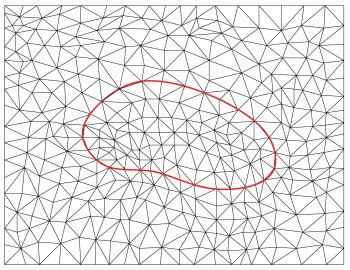
\includegraphics[width=0.4\textwidth]{gfx/immersed_boundary/general_partition_triangle.jpg}\label{fig:grid_f0}}
  \hfil
  \subfloat[unstructured body-fitted grid]{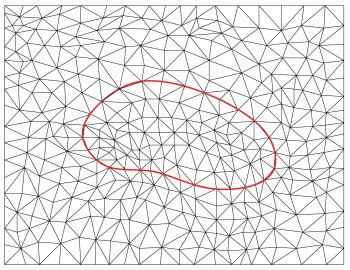
\includegraphics[width=0.4\textwidth]{gfx/immersed_boundary/general_partition_triangle.jpg}\label{fig:grid_f2}}
  \caption{Different types of numerical grids}
\end{figure}

For many fluid problems it is mandatory to solve the equations of motion with respect to complex-shaped geometries \.
The algorithm introduced in section () is not yet suitable for such a scenario.
For instance the simulation inside a spheric geometry is impossible, since the boundaries
do not coincide with the implemented cartesian grid. Nevertheless there exist different approaches to overcome this problem,
which shall be introduced here. \\
The common approach to extend the algorithm would be to use a body-fitted mesh (see figure \ref{fig:grid_f1}),
different advantages and disadvantages arise with this kind of implementation (see \citep{Mittal2005}).
One benefit is a much simpler deployment of the desired boundary condition, due to the overlap of the grid with domain border.
Furthermore a higher accuracy can be achieved \citep{Gornak2013}.
However, using an unstructered grid generates plenty of computational overhead, during and before the execution of a simulation.
The generation of the grid is very complicated in contrast to using a cartesian grid, this can be even more complicated when
considering moving boundaries.
Also solving the finite differenc schemes on a curvilinear coordinate system, leads to more calculations on a single grid point.
The last important aspect is the implementation on the gpu.
Like discussed in section () it is more efficient to use homogenous storage and calculation pattern on a CUDA-device,
the use of unstructured data makes this very difficult.
Altough some attempts exists to solve these difficulties (see i.e. PAP), it is still uncertain if the obtained performance loss would be acceptable.\\
A set of alternative methods, to resolve the problems described above, are so called Immersed Boundary Methods.
The term was first mentioned in (PESKIN 1972), for the simulation of blood flow through a heartvale, but has since then been used for a variety of
methods (MITTAL).  All of them have the idea in common to perform the simulations on a cartesian grid which does not conform to the domain boundary.
To satisfy the desired boundary conditions additional terms are introduced into the equations of motion.
In general one can distinguish between contiuous forcing methods and direct forcing methods.
Continious forcing methods try to mimic the boundary using a localized force which acts on the boundary,
since the surface is tracked by lagrangian points this methods can be well suited for moving boundaries (MITTAL).
One common problem is that continous forcing can arise to stability problem and numerical oscillations in numericial stiff problem (SOURCE).
The direct forcing approach tries to satisfies the boundary condition, by imposing it directly to points near the fluid surface for example
trough an interpolaltion procedure.
Some of the major drawbacks using the IBM is the loss in  spatial accuracy at the boundary, therefore it can be necessary to use a higher grid resolution
compared to a body-fitted mesh.  Futhermore the non-conforming (?) boundaries are more difficult implement.
The benefits of these methods is the use of a cartesian grid, which is much more suited for a gpu-based implementation (see section X).
As a result the overall performance will probably be in the same order as the original algorithm.
In the thesis the Implementation of different Immersed Boundary Methods is seperated into three chapters depending on the boundary condition and application.
This chapter beginns with Implementation of NoSlip-Walls which are the easisest to implement.
The term Immersed Boundary Method is vaguely defined in literature, in this thesis we refer to it with all methods introduced in the following three chapters.


\newpage

\section{Implemented Methods}

For the purpose of discussion, the different methods introduced here, will be applied to a default geometry.
The fluid domain without any immersed boundaries is set to a cube of the size $l_i= 1$ with  $i = \{x, y, z\}$.
For the discretization we choose $N_i = 32$ for the number of grid points.
As an example of an immersed boundary, we will dicuss the embedding of a cylinder, given by the  surface equation

\begin{align}
    \left(x - \frac{l_x}{2}\right)^2 + \left(y - \frac{l_y}{2}\right)^2 = r^2
\end{align}

where $r=0.4$ is the radius and the center is given by $(l_x/2, l_y/2)$. The whole setup is schematically shown in figure (X).
The simulation domain is than seperated into the fluid domain $\Omega_f$ and the wall domain $\Omega_w$.
The overall goal is to enforce the no-slip condition $\vec{v} = 0$ on the surface $\partial \Omega_f$, furthermore
the consveration of mass should be fulfilled.

\subsection{Volume Penalization}

\begin{figure}[!b]
    \subfloat[Cylinder geometry of the immersed boundary embedd in the simulation domain]{{
      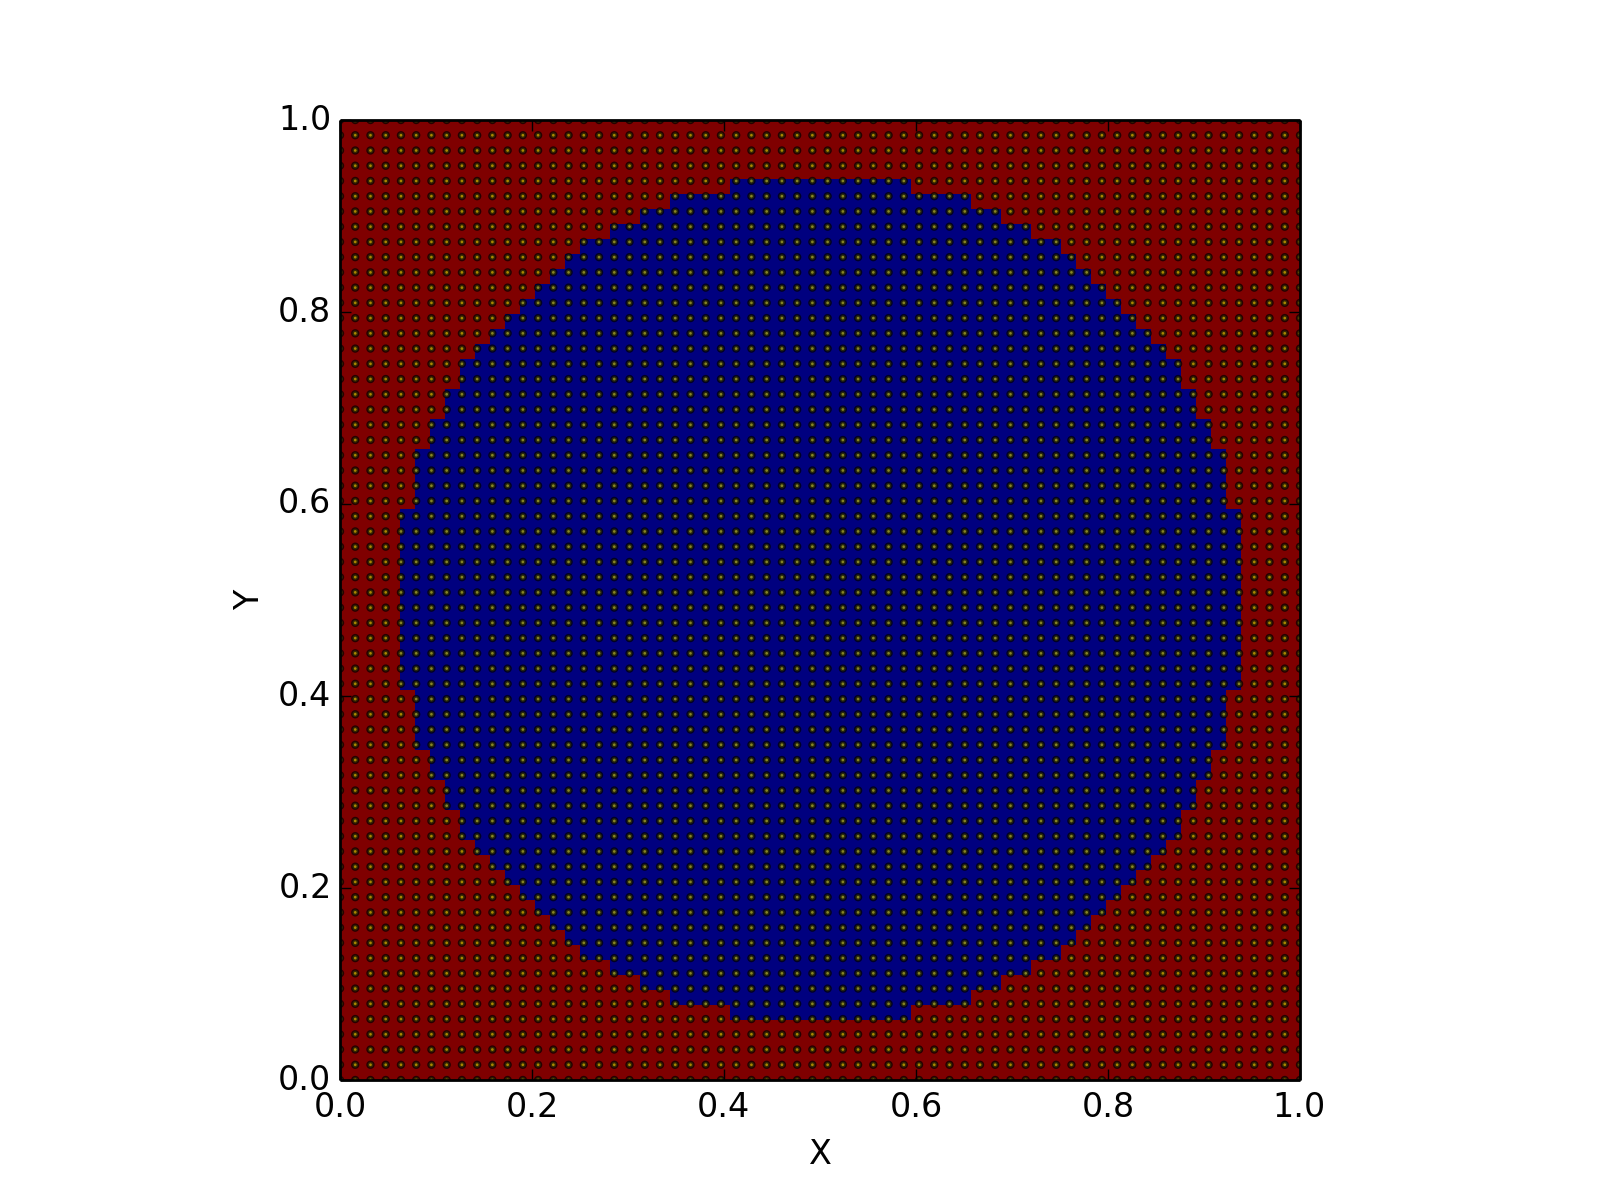
\includegraphics[width=0.5\textwidth]{gfx/immersed_boundary/mask.png}\label{fig:mask_vp}
        }}%
    \subfloat[Masking function $H(x,y,z=const.) = x^2 + y^2 < c$ for a cylinder. ]{{
      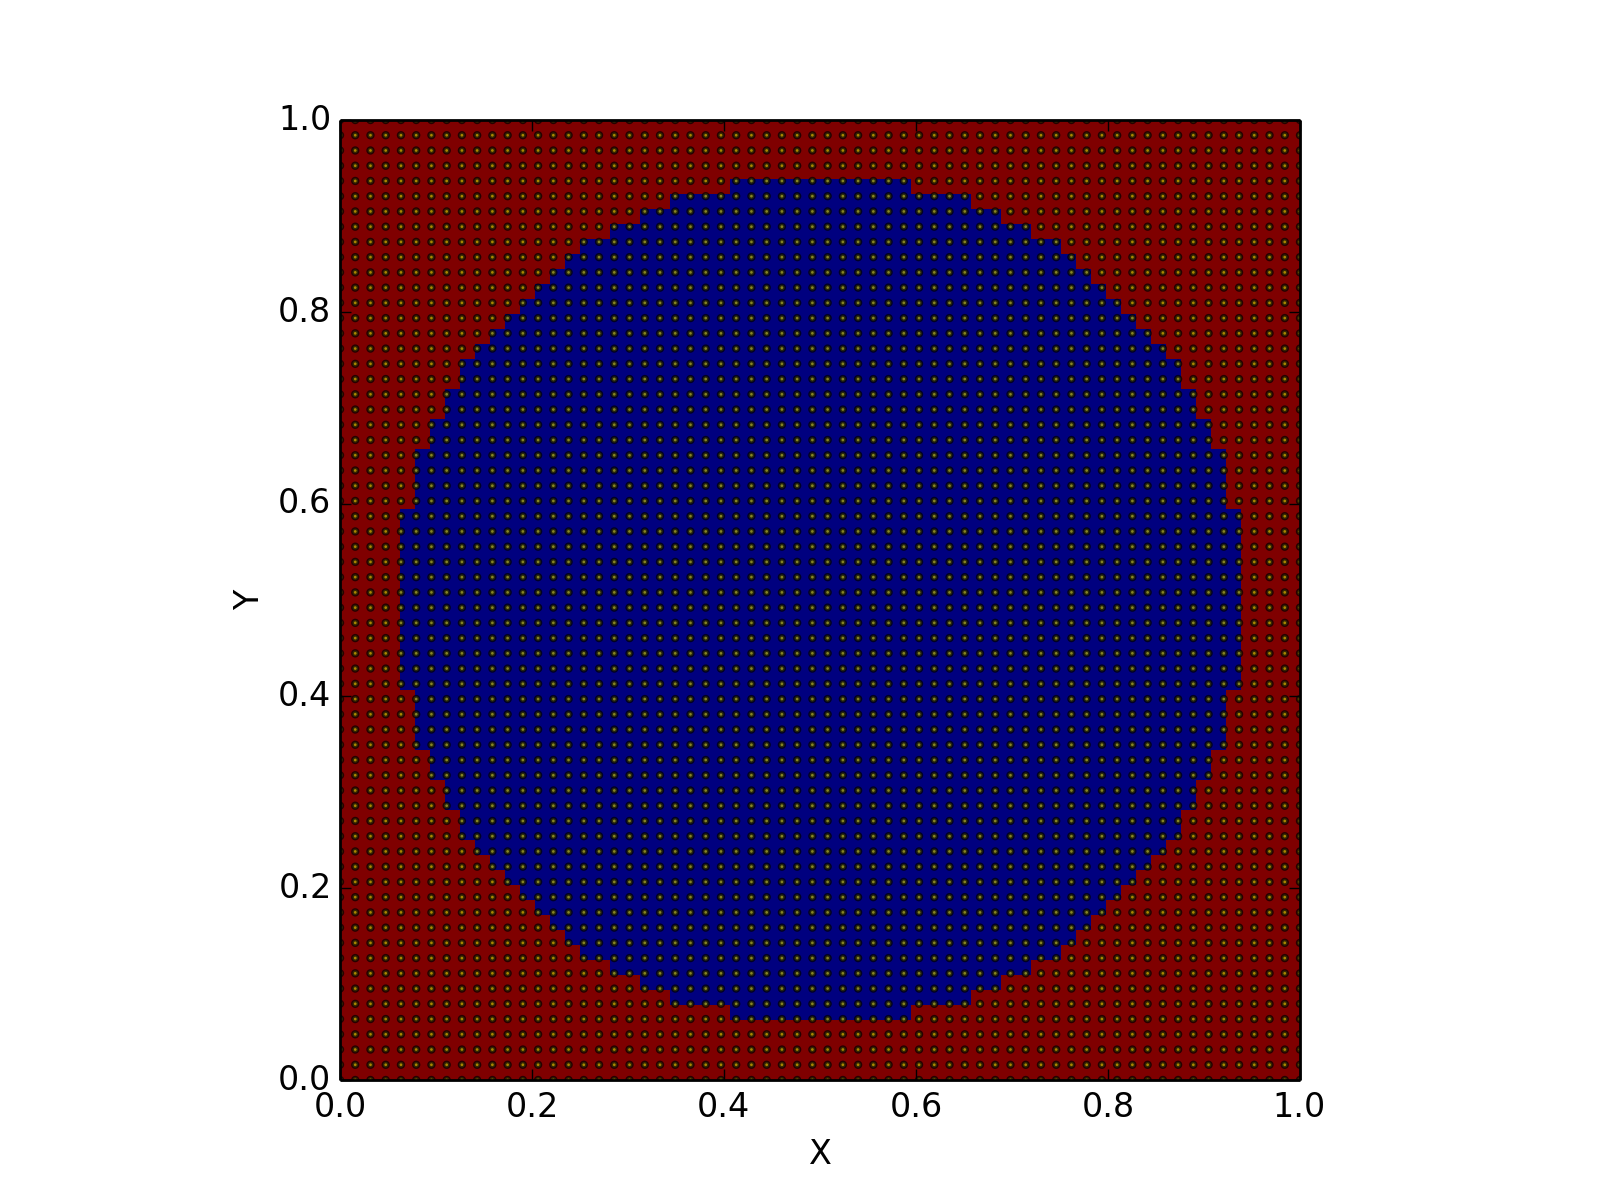
\includegraphics[width=0.5\textwidth]{gfx/immersed_boundary/mask.png}\label{fig:mask_vp}
     }}%
    \label{fig:example}%
\end{figure}

The idea behind the volume penalization method is to introduce an additional forcing term into the Navier-Stokes equation, which acts on
the grid points outside of the fluid domain to ensure the desired boundary conditions. The methods was sucessfully implemented and tested
on pseudo-spectral methods, see for example (CITE).
For the implementation it is necessary to define a masking function $H(x, y, z)$ which seperates the simulation domain into $\Omega_f$ and $\Omega_w$.
In case of the cylinder, we can use the surface equation (REF) and simply obtain.
\begin{align}
H(x, y, z) = \begin{cases}
                    0, &  \left(x - \frac{l_x}{2}\right)^2 + \left(y - \frac{l_y}{2}\right)^2 <r^2\\
                    1, & \text{else}
             \end{cases}
\end{align}
Now we can introduce an additional forcing term into the impulse equation,
\begin{align}
    \pdn[u]{t} + \vec{u} \cdot \vec{\nabla} \vec{u} &= -c^2 \nabla \rho + \frac{1}{Re} \Delta \vec{u} + \vec{F}_{ext}
     +\underbrace{ \frac{H(x, y, z)}{\nu}(\vec{v} - \vec{v_0})}_{\text{damping force}}
\end{align}

where $\vec{v}_0$ conforms the desired boundary condition, i.e. $\vec{v}_0 = 0 $ for no slip boundaries, and $\nu$ is a regulation parameter also denoted as damping rate of the forcing.
The additional term acts as an exponential damping force on a single gridpoint inside of $\Omega_w$, by the product with since it vanishes in $\Omega_f$ by the definition of $H(x,y,z)$.


Die Antwort des Kraftterms wird durch die Dämpfungrate $\nu$ reguliert. Je kleiner $\nu$ desto stärker ist die Dämpfungsrate, allerdings kann der Term
nicht beliebig klein gesetzt werden da die Stabilität für $\nu < dt$ nicht mehr gewährleistet ist [source].
Da für die Lösung der der Geschwindingskeitsfelder mit der Methode der künstliche Kompressibilität  bereits ein sehr kleiner Zeitschritt verwendet wird (s.Abb. X)
kann im Vergleich zu anderen Verfahren wie z.B. (pseudo-spektrale) eine relativ starke Dämpfungsrate verwendet werden.
-konvergenz nu gegen 0 MPI\\
- stiff probplem dt < dtpen = nu DIPLOM\\
- dary type law MPI\\
\newpage


\subsection{Direct Forcing}
Während die Volume Penalization Methode die Geschwindigkeit ausserhalb des Volumens nicht vollständig auf Null setzt,
 kann dies durch eine implizite Berechnung des Dämpfungsterm erreichtwerden. Es stellt sich heraus das dieser Ansatz equivalent
  zu der Direct Forcing Methode ist, die erstmals von [] verwendet und in [] beschrieben wird.
Betrachten wir zunächst den diskretisierten Zeitschritt
\begin{align}
    \frac{\vec{u}^{n+1} -\vec{u}^n}{\Delta t} = \mathscr{L} + \vec{f}\\
\end{align}
wobei $\mathscr{L}$ den diskretiesierten Operatoren der PDE entspricht.
Für einen Punkt auf dem Rand des Volumens soll nun die Randbedingung $\vec{u}^{n+1} = \vec{u}_0$ eingehalten werden.
Mit Formel () folgt
\begin{align}
    \frac{\vec{u}_0 -\vec{u}^n}{\Delta t} = \mathscr{L} + \vec{f} \Rightarrow \vec{f} = \frac{\vec{u}_0 -\vec{u}^n}{\Delta t\cdot \mathscr{L}}\\
\end{align}

Mit der Annahme dass der Rand mit dem numerischen Gitter übereinstimmt ist es nicht nötig den Kraftterm zur berechnen, stattdessen lässt sich der
Schritt vereinfachen in dem der Randwert nach  jedem Zeitschritt direkt auf die gewünschte Randbedingung gesetzt wird. Durch die
implizite Behandlung kommt es zu keiner weiter Stabilitätsbedingung.

\newpage

\subsection{Volume Fraction Interpolation}

The methods introduced up to here lack the ability of an exact impementation of the boundary conditions on $\Omega_f$.
Instead the surface $\partial \Omega_f$ is described by the nearest grid points in $\Omega_w$, resulting in an
stepwise approximation.
To overcome this problem a simple procedure is the use of an volume fraction interpolation scheme, introduced in [FADL].\\
The advantage of this method is the simple implementation into the volume penalization and direct forcing method.
Furthermore the overall computation time of the timestep stays constant, in  contrast to complex interpolation schemes.\\
Initially the interpolation beginns by determine all grid cells\footnote{definition cell} which are cut by the surface $\partial \Omega_f$.
For each of these boundary cells the total volume $V_w$ of the wall domain $\Omega_w$, inside each cell, is computed.
The force acting on the points inside the boundary cells is than weighted by a scaling factor, $\Phi = V_W/(\Delta x \Delta y \Delta z)$.
For the volume penalization method the scaling is simply multplied with the forcing term in eq. ().
Since the implementation of the direct forcing method is setting the velocity components directly to zero, it is necessary to
fall back to equation () and introduce a forcing term

\begin{align}
    \vec{f} = \Phi \frac{\vec{u}_0 -\vec{u}^n}{\Delta t\cdot \mathscr{L}}\\
\end{align}

\begin{figure}[!bp]
    \centering
    \subfloat[label 1]{{
      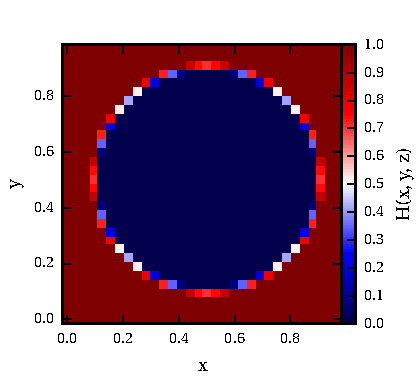
\includegraphics{gfx/immersed_boundary/methods/mask_volfrac.pdf}\label{fig:mask_volfrac}
        }}%
    \qquad
    \subfloat[label 2]{{
      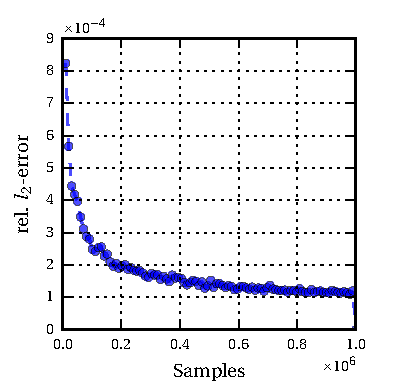
\includegraphics{gfx/immersed_boundary/methods/error_volfrac.pdf}\label{fig:error_volfrac}
        }}%
    \label{fig:example}%
\end{figure}

Since the operator $\mathscr{L}$ is computed during the first part of the time step. This forcing term can added during the completion of the runge kutta step.\footnote{see section}\\
For the implementation of an extended version of the masking array $H$ is used.
Like in the previous methods the masking array is precomputed and loaded at runtime. The algorithm is extended to compute the
volume fractions of the cells lying next to the surface $\partial\Omega_f$.
Since an exact computation is difficult to implement for abritary surfaces, the idea is to use a monte carlo integration method.
For each cell $N$ random samples are generated, then the volume fraction is simply given by the ratio of samples lying in- and outside ot the domain.
The implementation into a simulation class using the python API is explained in more detail in Appendix ().\\
An example for the computed masking array with $N=2e5$, is shown in figure (). The symmetric distribution of the boundarie values indicates
a good approximation, for a better evaluation a convergence study was performed were the number of samples $S$ was varied between 100 and $10^6$ points.
The $l_2$-error was determined by comparing the results to the computation with the highest number of samples.
The results are shown in figure ().\\

-discussion for n>10000 error 1e-5\\
-overall good approximation \\
-erweiterung  *2 etc blabla\\



\subsection{Interpolation}
\newpage

\section{Validation}

In order to ensure a correct numerical behaviour of the introduced methods,
a large part of the thesis deals with the numerical validation.
Multiple examples from simple to more complex testcases are introduced in this section.
In general it is necessary to obtain a good evaluation of the numerical truncation error, the numerical stability over longer periods of time
and the fullfilment of the conversation laws, most importantly mass conservation.
Grid convergence studys against theoretical and high-resolution numerical solutions  will be performed
and compared for the different IBMs.


\subsection{Laminar Poiseuille-Flow}
\subsubsection{Theoretical description}

\begin{figure}[!bp]
  \centering
  \includegraphics[width=0.8\textwidth]{gfx/immersed_boundary/val_volpen/poiseuilleflow.png}\label{b}
  \caption{Theoretical setup of the poiseuille-flow channel.}
\end{figure}

%\begin{wrapfigure}{r}{0.5\textwidth}
%  \begin{center}
%      \includegraphics[width=0.48\textwidth]{gfx/immersed_boundary_methods/val_volpen/poiseuilleflow.png}
%   \end{center}
%          \caption{ paxvleb xvle}
%\end{wrapfigure}


The first testcases is the laminar poiseuille-flow, the theoretical setup is presented in figure ().
It consist of two infintiy long planes at $z=h_1$ and $z=h_2$, which are oriented parallel to the xy-plane and the distance $\Delta h = h_2 - h_1$ between them.
Numerically this is realized by using periodic boundaries in xy-direction and no-slip boundaries in z-direction.
The velocity profile results from an external force, given by a  pressure gradient in x-direction, which is introduced into the naviers-stokes equation.
No other forces are present furthermore the flow will be independent of the y coordinate,
hence for the steady state $\partial v_x /\partial t = 0$ the equations of motion can be reduced to:

\begin{align}
\frac{\partial v}{\partial t} &= - \frac{\partial p}{\partial x} + \nu \frac{\partial^2 v_x}{\partial z^2} = 0
\end{align}

where v is the velocity in x direction.
For the non-dimenzionalization we choose $r^* = r/L$, $v^*=v/L$, $t^* = \frac{V}{L}$ and $p^* = p \rho V^2$ where $L=\Delta h$ and $V=v_{max}$.
The non-dimensional equation reads

\begin{align}
\frac{\partial v}{\partial t} &= - \frac{\partial p}{\partial x} + \frac{1}{Re} \frac{\partial^2 v_x}{\partial z^2} = 0
\end{align}

with $Re = VL/\nu$.
For the volume penalization method we furthermore obtain a non-dimensional damping force $-\frac{H}{J}\cdot v$ with $J = VL/\eta$.
The equation can simply be integrated twice which yields the solution

\begin{align}
v &= \frac{1}{2}\frac{\partial p}{\partial x}z^2 + zc_1 + c_2
\end{align}

Using the noslip-boundary condition $v_x(h_1) = v_x(h_2) = 0$ and furthermore by defining
$A:=\frac{1}{2}\frac{\partial p}{\partial x} Re$ one obtains the additional conditions

\begin{align}
c_1 &= A\frac{h_1^2 -h_2^2}{h_2 - h_1} = -A(h_1+h_2)\\
c_2 &= A(h_1(h_1 + h_2) - h_1^2) = Ah_1h_2\\
\end{align}

The velocity is than given by the quadratic function

\begin{align}
v_x &= A(z^2 - z(h_1 + h_2) + h_1h_2)
\end{align}

The maximum velocity and postinon can be obtained by simple calculus

\begin{align}
z_{max} &= \frac{h_1+h_2}{2} \wedge v_{max} = A\left(h_1h_2 - \frac{(h_1 + h_2)^2}{4}\right)
\end{align}

Since $v_{max}$ has to be 1 by definition of the non-dimensionalzation we find

\begin{align}
\frac{\partial p}{\partial x} &= \frac{2}{Re}\frac{1}{\left(h_1h_2 - \frac{(h_1+h_2)^2}{4} \right)}
\end{align}

as a necessary condition for the pressure gradient.\\
With the given theoretical solution, the next objective is the comparison
to the default implementation, the volume penalization method and the direct forcing method.
Since we have a flow parallel to the grid  it does not make sence to compare it to the interpolation methods
For the comparision with a theoretical solution it is necessary to ensure that the surface grid points match with the total height $h$ of the channel.
In the default setup tes gibthe noslip-boundaries are realized with the default implementation, like explained in section ().
For the immersed boundary methdos the upper- and lower boundaries are given by the masking function.
\begin{align}
H(x, y, z) = \begin{cases}
                    0, & \text{for \  }  z < h_2 \lor z>h_1 \\
                    1, & \text{else}.
             \end{cases}
\end{align}

\subsubsection{Test of the Default Implementation}

\begin{figure}[!bp]
    \centering
    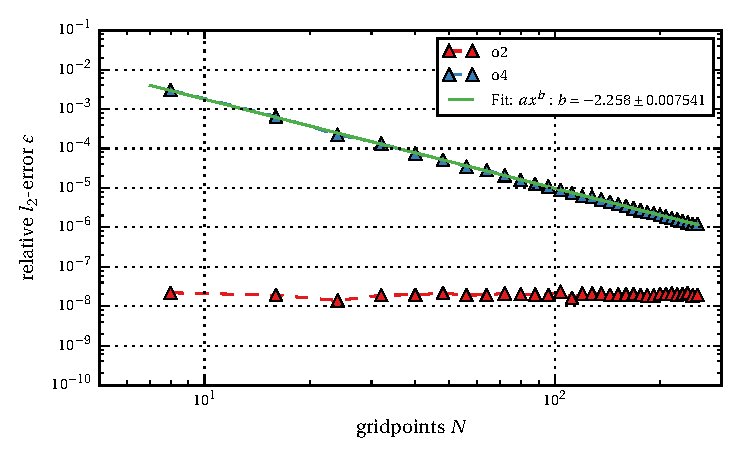
\includegraphics{gfx/immersed_boundary/poiseuille_flow/1_default/relative_l2error.pdf}
    \caption{Relative $l_2$-error for second and fourth order schemes of the default algorithm.\label{fig:ema1}}
\end{figure}

Initially a grid convergence test was performed with the default implementation of the algorithm, without the use of immersed boundaries.
For this test case this is still possible since the geometry is non-curved and parallel to the cartesian grid.\\
For the  numerical setup the parameters were set to $l_x=1$, $l_y=0.25$, $l_z=1$.
The reynolds number was set to a constant value of $Re=500$, whereas the resolution $N$ was varied in the Intervall $[16 - 128]$ with a stepsize of $\Delta N = 8$.
The timestep was set to $\mathrm{dt}=1e-5$ and the pressure gradient to $\partial p \partial x  = 10$.
For all resolutions the simulations were performed for finite differcen schemes of second and fourth order.
The results are shown in figure \ref{fig:ema1} on a double logarithmic plot.\\
For the finite difference scheme of second order, the error behaves not as assumed.
Instead of the decline one would expect with the decrease of the resolution, the  error is nearly constant.
This behaviour can be explained due to the lack of complexity of the test case. As the theoretical solution is a polynom of second order
no higher order terms will occur in the numerical solution, hence the second order scheme is capable of a perfect approximation, independent of the
grid resolution. The remaining error terms, are of the order $10e^{-8}$, which is extremly small and occur due to the floating point round off.
With this in mind the behavior of the fourth-order scheme is even more unexpected.
We see a linear decrease of the error on the log scale.
The result of a power law fit yields a convergence rate of second order.
Furthermore the error is much larger compared to the second order scheme, there is a decrease from $10e^{-2}$ to $10e^{-5}$.
The test case reveals that an error exists in the default implementation of the boundarie conditions.
An explanation can be given with comparison of the theoretical solution. The laplace operator is given by
 $ \nu \pdn[^2 v_x]{x^2} = 2A = \frac{1}{\nu}\pdn[p]{x}$
Using the mirroring method creates a discontinuous function at the boundaries, since the laplace operator changes the sign.
When using the second order method the tree-point-stencil evaluates to the correct value $\pdn[^2 v_x]{x^2} = 1$.
The five-point-stencil of the fourth orderer scheme evaluates to $\pdn[^2 v_x]{x^2} = 1$, since it uses one point behind the boundary.
As a result the discontinuity creates an error in the higher order scheme.\\
For this testcase the second order method yields better results, however we
have to keep in mind that the testcase yields a polynomial solution,
it is not clear how the results will end up for a complex testcase.
Furthermore in this testcase the boundaries have a large impact since the pressure gradient is parallel to wall,
his is not the case in general.
One possibility to avoid this error, would be to use an asymmetrich stencil, this approach is discussed in section ().

\begin{figure}[!b]
  \centering
  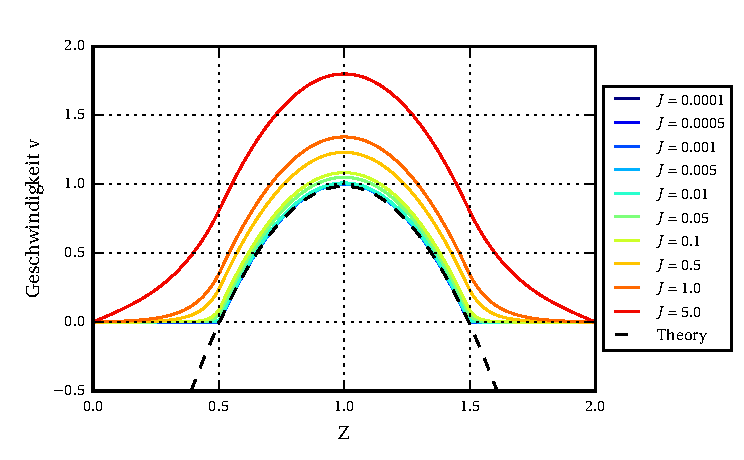
\includegraphics{gfx/immersed_boundary/poiseuille_flow/2_vp/vp_profile.pdf}\label{fig:vp_flow}
  \caption{Geschwindigkeistprofile im Kanal bei Variation der Dämpfungskonstante $\nu$ und Reynoldszahl $Re=500$.}
\end{figure}

\subsubsection{Test of the Volume Penalization Method}

The next objective is to investigate the error of the volume penalization method.
For this method the additional forcing term REFHERE is introduced into the equations. The non-dimenzionalzation leads to the form
\begin{align}
    \vec{f} = \frac{H}{J}v
\end{align}

with the quantity $J = 123$ as a non-dimensional forcing parameter.
(MACH NUBMER DISCUSSION HERE) \\
We begin by studying the behavior of the velocity profile, with variation of the Reynolds-number and the damping $J$, in the regime $Re=100-500$ and $\nu=1e-4 - 5e-1$.
The numerical setup is equal to the one for the default methods, except we now introduce the masking function (LABELABOVE) with $h_1=0.25$ and $h_2=0.75$.
To make sure that the channel width is equal to $\Delta h = 1$, the total height was set to $l_z\approx2.01587$. This furthermore ensures that the grid points overlap exactly
with the masking function at $h_1$ and $h_2$. The resolution was set to $N_x\times N_y\times N_z = 64\times16\times128$.
The resulting velocity profile is exemplarily shown in figure \ref{fig:vp_flow}, for varying $\nu$ and a constant reynolds number $Re=500$, for the second order scheme.\\
It can be noted that with an decrease of $\nu$, the numerical solution converges against the theoretical one.
The quadratic part of the velocity profile inside the fluid domain is independent of the damping constant $\nu$.
Since the damping can not fullfill the exact boundarie conditions, a slight offset is introduced into the velocity profile
which leads to an offset in the solution.
In the masked area of the volume we can see an exponential decrease of the total velocity.
Since for the steady state

\begin{align}
 \nu v &= D \frac{\partial^2 v_x}{\partial z^2}  \Rightarrow  v_x = A e^{\sqrt{\frac{\nu}{D}}v_x}
\end{align}

where A is given by the offset $v(h_1)$.\\
For an error estimation, the relative $l_2$-error was computed.
The results for the second order scheme are shown in figure \ref{fig:vp_error}.

\begin{figure}[!t]
  \centering
  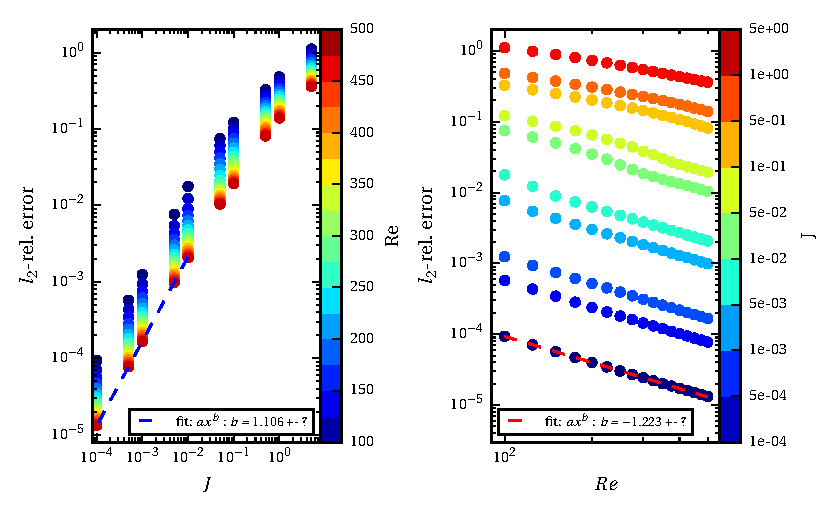
\includegraphics{gfx/immersed_boundary/poiseuille_flow/2_vp/vp_error.pdf}\label{fig:vp_error}
  \caption{Relative $l_2$-error for variable damping rate $\nu$ and reynolds-number $Re$.}
\end{figure}


The error decreases together with the damping rate from $1e-0$ to $1e-4$. For $nu<1e-3$ and a constant reynolds number we can observe an almost linear decrease in the logarithmic space,
this yiels a fit law of the form $ e = ax^b$. This shows that the error of this penalization method converges with first order in dependence of $\nu$.
The decrease for $nu>=1e-3$ can be explained by having a look at figure \ref{fig:vp_flow} again. Since the damping in the masking area is to
weak the flow sees the real boundaries of the fluid domains, which results in a stronger damping on the flow.
This is not the case for $nu<1e-3$ since the velocities reaches zero before reaching the boundarie.\\
Furthermore we can see a decrease of the error of one order with an increase in the reynolds number.
Since the damping force is proportional to the velocity and therefore to the reynolds number, the offset on the channel walls remains constant.
Due to the larger velocity profile this results in an smaller relative $l_2$-error, whereas the absolute error will increase.
For the fourth order scheme, the error is shown in figure APPENDIX.
We can observe a similar convergence  until the damping rate decreases to $\nu=1e-4$, below that value the error increases slightly to the order of magnitude of $1e-3$.
The reason for this behavior will be discussed soon.\\
Finally a grid convergence study was carried out, with a constant Reynolds number and $\nu \in [1-23]$.
The resolution was varied between $N\in [4, 400]$ with $\Delta N = 4$, second and fourth order schemes were tested.
For the correct solution the theoretical velocity profile (REF) was assumed.
The results are shown in figure().

\begin{figure}[!t]
  \centering
  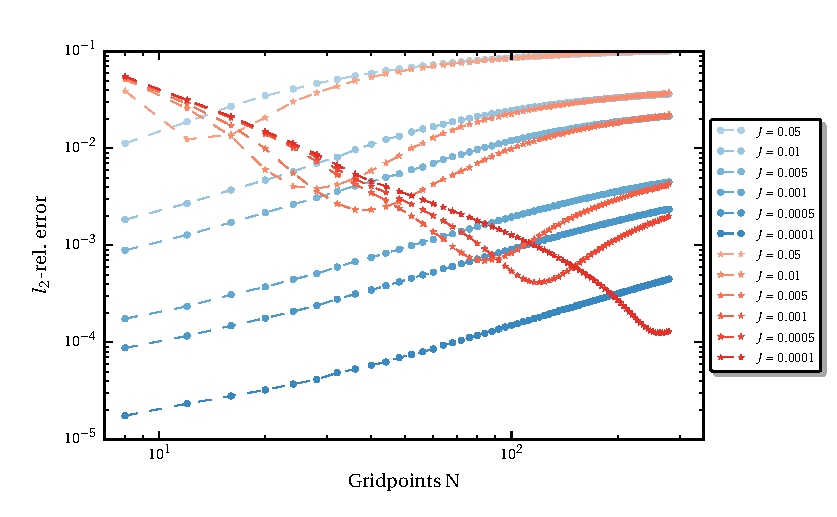
\includegraphics{gfx/immersed_boundary/poiseuille_flow/2_vp/vp_convergence.pdf}\label{fig:vp_conv}
  \caption{Absoluter und relativer Fehler in Abhängigkeit von Dämpfungskonsante $\nu$ und Reynoldszahl $Re$.}
\end{figure}
One can observe again that a decrease in $\nu$  yields a smaller error.
For the second order scheme we can see that with an increase in the resolution, the error increases and finally converges against a constant value.
Even more confusing is the behaviour for the fourth order scheme.
With increasing resolution we can see a decrease into a local minimum, followed by an increase to the same error as the second order scheme.
An explanation of this behaviour can by given by revising the theoretical solution and the finite difference stencils at the immersed boundary.

The error does not converge towards zero, which means there has to be some discrepancy to the theoretical solution.
For a constant $\nu$ there is an offset to the theoretical solution, which we allready saw in figure (REF).
Hence by increasing the resolution the numerical solution converges towards the wrong solution.
The error increases since for a lower resolution, the velocity profile is closer to the assumed theoretical for the second order method.

\begin{align}
 \nu v &= D \frac{\partial^2 v_x}{\partial z^2}  \Rightarrow  v_x = A e^{\sqrt{\frac{\nu}{D}}v_x}
\end{align}
\begin{figure}%
    \centering
    \subfloat[label 1]{{
      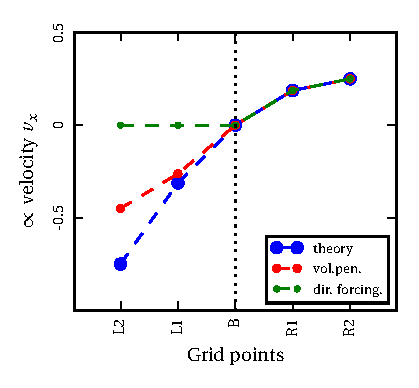
\includegraphics{gfx/immersed_boundary/poiseuille_flow/extra/stencil.pdf}\label{fig:mask_vp}
        }}%
    \qquad
    \subfloat[label 2]{{
      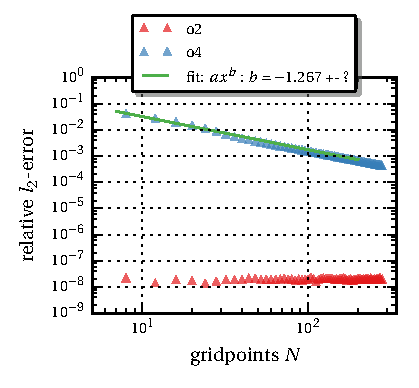
\includegraphics{gfx/immersed_boundary/poiseuille_flow/3_df/relative_l2error.pdf}\label{fig:mask_vp}
        }}%
    \label{fig:example}%
\end{figure}


The explanation for the fourth order convergence has again to do with the discretization error at the boundary.
Figure () shows schematically the velocity profiles for the volume penalizaton method compared to the theoretical.
Due to the different  profiles, the numerical evaluation of the laplace operator results
into different friction rates for the border point \textbf(B), but  also for the first next neighboor in the fluid domain \textbf(R1) when fourth order schemes are used.
For the fourth order scheme the laplace operator at the boundary evaluates to a slightly (CALCULATE) negative value), which means the friction at the boundary due to
viscosity is stronger. The result is a smaller velocity profile which when increasing the resolution starts to overlap best with the theoretical solution at the minimal error.
Finally when increasing the resolution further the error increases since the method converges towards the same resolution as the second order scheme (IMAGE MAYBE?).
An attempt has been made to fit the numerical solution to a quadratic profile for the comparision to a theoretical solution but this didn't work due to blabla
(FIT IDEA NOT WORKING CONVERGENCE AGAINST HIGH RESOLUTION.

\subsection{Direct Forcing Method}

For the comparsion to the direct forcing method another grid convergence study was carried out.  As a parameter we used same as above, the results are shown in figure X.
-We can see o4 not working reason is the same as we can se in figure n) , the laplacian is wrong caclulated at the point B.
As a results an error is induced at the boundaries of the domain.
The second order scheme works perfectly as we compare it to the default implementation.

\subsection{Poiseuille Flow with variable pressure gradient}

Finally

\begin{align}
\frac{\partial p}{\partial x} &= P_0 \sin(\pi n z)
\end{align}

solution with the same non-dimensionalization yields

\begin{align}
 \nu v &=  \sin(\pi n z)
\end{align}

with the condition

\begin{align}
 P_0 &= -\frac{\pi^2n^2}{Re}
\end{align}

to satisfie $v_{max} = 1$.


\begin{align}
 \nu v &= D \frac{\partial^2 v_x}{\partial z^2}  \Rightarrow  v_x = A e^{\sqrt{\frac{\nu}{D}}v_x}
\end{align}
\begin{figure}%
    \centering
    \subfloat[label 1]{{
      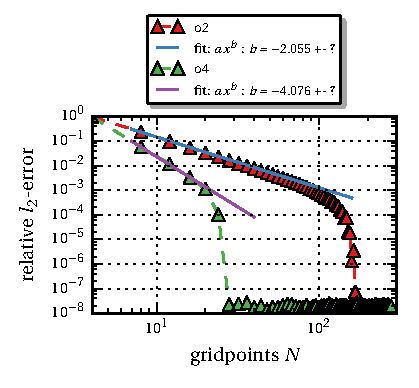
\includegraphics{gfx/immersed_boundary/poiseuille_flow/4_sine/relative_l2error.pdf}\label{fig:mask_vp}
        }}%
    \qquad
    \subfloat[label 2]{{
      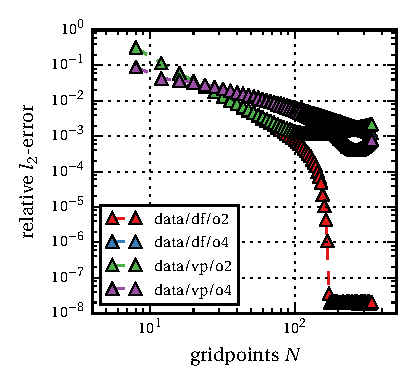
\includegraphics{gfx/immersed_boundary/poiseuille_flow/4_sine/relative_l2error_methods.pdf}\label{fig:mask_vp}
        }}%
    \label{fig:example}%
\end{figure}

\newpage
\subsection{Hagen-Poiseuille Flow}

\subsubsection{Theoretical description}

In the previous testcase the channel walls were aligned parallel to the simulation grid, hence no further interpolation procedures
were necessary. In order to test the accuray of the interpolation methods, we now introduce a testcase with a curved geometry.
Furthermore we have the possibility to investigate the error of non-interpolating methods on curved surfaces.\\
The most simplest extension of the planar poiseuille flow, is the laminar flow through a pipe,
also referred to as Hagen-Poiseuille flow. The setup of the fluid domain is schematically shown in figure ().
We consider a flow in z-Direction where the total size of the simulation domain is set to $L_x = L_y = L$.
The immersed boundary is restricted by a wall at the radius $r_0=0.4L$ where r is defined as the distance from the pipe center $\vec{m} = (L/2, L/2)^T$.
The length $L_z$ can be chosen arbitrary due to the flow invariance in z direction.\\
\begin{figure}[!bp]
  \centering
  \includegraphics[width=0.8\textwidth]{gfx/immersed_boundary/val_volpen/poiseuilleflow.png}\label{b}
  \caption{Theoretical setup of the poiseuille-flow channel.}
\end{figure}
For an analytical solution of this problem we referr to [CITEFLUID].
Once again we can assume a steady state flow which implies $\partial v_z/\partial t = 0$. With the introduction of cylindrical coordinates $(r, \phi, x)$
and the assumption that the flow is independent of $\phi$ the equation of motion reduces to
\begin{align}
        0 &= - \frac{\partial p}{\partial x}  +  \frac{\nu}{r}\frac{\partial}{\partial r}\left(r\frac{\partial u}{\partial r}\right)
\end{align}
The solution is obtained by seperation of variables and integrating twice.
\begin{align}
    u &= \frac{r^2}{4\nu}\frac{\partial p}{\partial x} + A \ln r + B
\end{align}
By using the boundarie conditions $u(r_0) = 0$ and choose the same non-dimensionalization as in section (), with the expection of setting the length scale to $r_0$,
the velocity profile for the channel is given by
\begin{align}
    u &= \frac{r^2 - r_0^2}{4}\frac{\partial p}{\partial x}Re
\end{align}
Since $v_{max} \stackrel{!}{=} 1$ by definition, the pressure condition for the domain needs to be set to
\begin{align}
    \frac{\partial p}{\partial x} = -\frac{4 r_o^2}{Re}
\end{align}

\subsubsection{Grid Convergence Study}

For an error evaluation a grid convergence study was performed, for a constant reynolds number of $Re=100$.
The number of grid points was varied in the intervall $N\in[32, 256]$ with a stepsize of $\Delta N = 16$, furthermore a
simulation with a resolution of $N=512$ was carried out.\\
Since the maximum velocity of the channel is given by $v_{max}=1$, due to the choice of non-dimensionalization,
the sound speed was set to $c^2 = 100$ to fullfill the incompressibilty condition $Ma = v/c < 0.1$. \footnote{In order to exclude
any influence of choice of the sound speed on the resulting error, further simulations were carried out with a diffent $c^2$ and will be discussed}
With this choice the cfl-condition for the system is given by $\Delta t < \min(\Delta x^2 \cdot Re, \Delta x / 10)$.
The resulting timestep for the highest resolution is $\Delta t = 1e-4$.
With the above defined setup all methods introduced in section were tested, for second and fourth order finite difference stencils.\\
For the penalization method the non-dimensionalized damping was set to $J=1e-4$.
It would be possible to choose a larger time step for the lower resolution cases, which means that in general
one would apply a smaller damping rate $J$ in a case of applicaton. To remain consistent in the error convergence, here $J$ and
therefore $\Delta t$ was not altered.\\
The results of the computation are shown from figure () to figure().
In figure (X) the relative $l_2$-error is shown for the volume penalization method with and without the volume fraction method
for second and fourth order. The modified volume fraction method is not present since the computed error is almost identical to the default method,
such that the values overlap in the plot.

\begin{figure}[!pt]
  \centering
  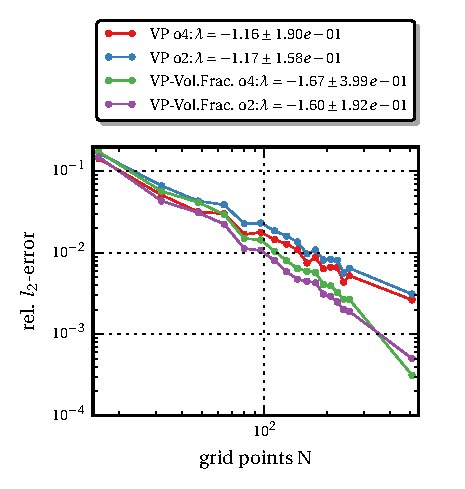
\includegraphics{gfx/immersed_boundary/hpflow/theo/vp.pdf}\label{fig:hpflow_vpgc_theo}
  \caption{blabla}
\end{figure}

\begin{figure}[!pb]
  \centering
  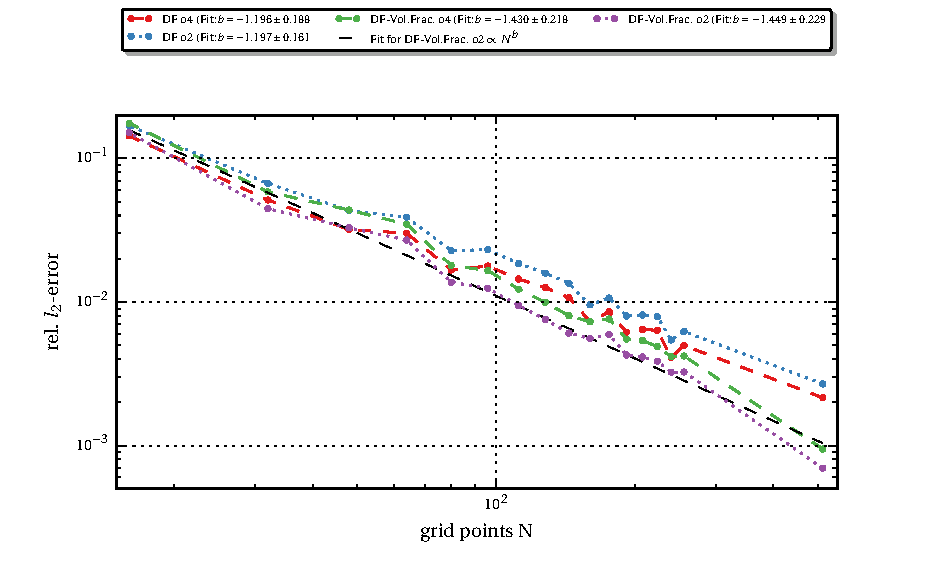
\includegraphics{gfx/immersed_boundary/hpflow/theo/df.pdf}\label{fig:hpflow_dfgc_theo}
  \caption{blabla}
\end{figure}


\begin{figure}[!pt]
  \centering
  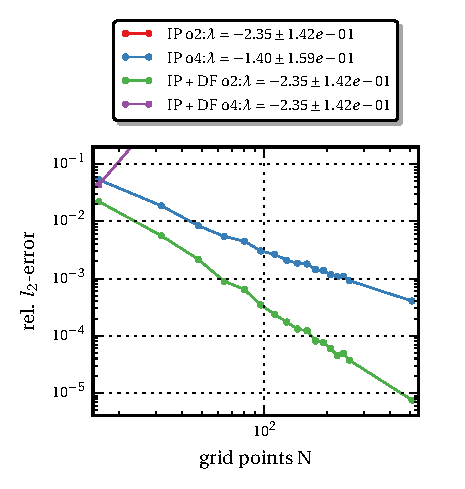
\includegraphics{gfx/immersed_boundary/hpflow/theo/ip.pdf}\label{fig:hpflow_ipgc_theo}
  \caption{blabla}
\end{figure}

\begin{figure}[!pb]
  \centering
  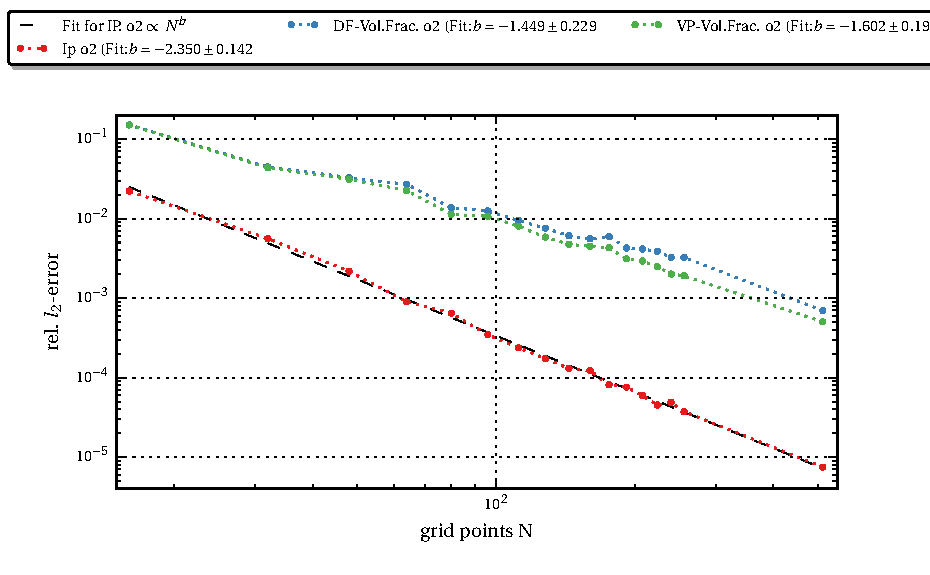
\includegraphics{gfx/immersed_boundary/hpflow/theo/all.pdf}\label{fig:hpflow_allgc_theo}
  \caption{blabla}
\end{figure}

\newpage

For all methods an approximately linear decrease  can be observed.
The error of volume penalizations methods decrease from the order $1e-1$ to $2e-3$, with
a convergence rate of order  $\epsilon \propto N^{\approx1.16}$
The volume fraction methods results in a slighty better convergence rate of $\approx 1.65$.
The overall error is smaller, due to the faster converge rates and of order $5e-4$ for the
highest resolution. For all methods the error is in the order of $1e-2$, above a resolution of 100 points.
The best results are achieved for the second order volume fraction method, except for the highest resolution.\\
Figure () shows the error of the Direct Forcing method with and without the volume fraction method for second
and fourth order. The error convergence is almost identical to the volume penalization method, when not using the volume
fraction method, of the order $\approx 1.2$. The convergence of the volume fraction methods is of order $\approx 1.45$
and therefore slighly weaker the for the volume penalization method.
As before the best error convergence is given by the volume fraction methond of second order.\\
In Figure (X) we can see the error convergence of the interpolation schemes.
Here we used second and fourth order schemes, furthermore we compare the interpolation with and without the
use of the direct forcing method.
The fourth order interpolation with direct forcing is not shown, since the resulting velocity fields are becoming
numerically unstable. The fourth order interpolation without DF also results into a larger error but in this case
the velocity field seems to be stable \footnote{This behaviour will be discussed in more detail in section ()}, the
convergence rate is of order $\approx 1.4$ and the error in the regime $1e-1$ to $4e-3$.
The best and furthermore identical results are achieved for the second order interpolation with and without
use of the direct forcing method. The convergence rate is of order $\approx 2.35$ and the error
decreases from the order $2e-2$ to $1e-5$. The identy of these methods occurs due to the decoupling of the velocity fields
on the border ot the fluid domain. Since the interpolation stencil seperates the fluid and wall domain, the second order
stencil doesn't see any points in the wall domain, therefore there is no difference in using the direct forcing method.\\
Finally figure () shows the previous methods with the best convergence rates in one plot.
In summary we can say that the overall converges rate of the interpolation method is of one order better
than the volume and direct forcing methods with volume fraction. Furthermore the relative error of the interpolation method ranges
between one and two order of magnitudes below all other methods, depending on the resolution.
The grid convergence study was than repeated once again in order to test the influence of the sound speed with $c^2 = 400$.
As a result it turned out that for all methods the difference in the relative $l_2$-error can be neglected, except
for the fourth order interpolation schemes, in this case the overall error grows. An exemplary plot which compares
the error can be found in Appendix in figure (). This behaviour indicates that when using the interpolation with fourth order
an error is induced which is proportional to $c^2\nabla \rho$.\\
As we allready could observe in section (), each immersed boundary method does not converge against the exact theoretical solution.
Therefore, for each method, a grid convergence study was peformed where the theoretical solution is given by a
high resolution solution of each method with $N=512$ points. This type of grid convergence study is often proposed
when no theoretical solution of the fluid problem can be achieved (SOURCE).
For this kind of grid convergence study the numerical setup is similar to the previous one with exeption of the resolution.
Here we use $N\in\{16, 32, 64, 128, 256\}$ for the number of grid points.
The problem occuring with other types of resolution is the position of grid points, which would not exactly overlap anymore with
the high resolution grid  of the theoretical solution of $N=512$.
An alternative would be to use interpolation methods for the exact positions, but the possible disadvantage with these method
would be an additional error resulting from the interpolation scheme.\\
The results of the error analysis are shown in figure () (a), exemplarly for the volume penalization, direct forcing  methods with volume fraction
and the interpolation method.


\begin{figure}[!pb]
  \centering
  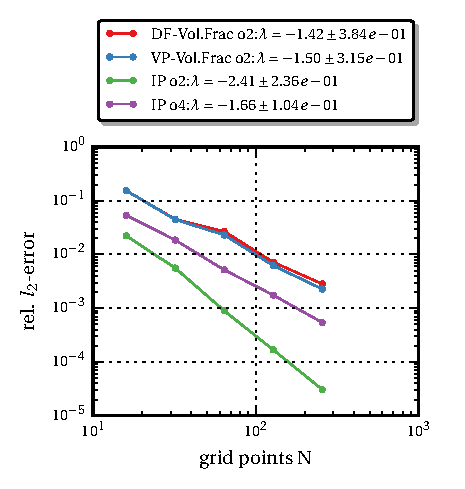
\includegraphics{gfx/immersed_boundary/hpflow/hd/all.pdf}\label{fig:hpflow_allgc_theo}
  \caption{blabla}
\end{figure}

-volfrac und dfrac bad convergence
-ip o4 ohne set zero wegen rho error rand
-ip 02 gut oder fit ?
\newpage

\subsubsection{Long-Term Simulations}

In Order to test the  numerical stability, additionally a long-term simulation was performed for each IBM.
Again a Reynolds number of $Re=100$ was chosen, with a fixed resolution of $N=96$ grid points.

\newpage

\subsection{Taylor-Couette Flow}

-introduction

\subsubsection{Theoretical description}

blub blub
